% !TEX root = Theo_III.tex
\chapter{Magnetostatik}


In den vorigen Kapiteln haben wir uns mit der Elektrostatik beschäftigt und gesehen, wie Ladungen dem Coulombgesetz gehorchen und ein elektrisches Feld hervorrufen, das die Grundgleichungen $\rot \vec {E}=0$ und $\divg \vec {D}=0$ erfüllt.

In der Magnetostatik betrachten wir jetzt stationäre (also nicht zeitabhängige) Ströme und die Kraftwirkung, die sie hervorrufen. Es wird ein Magnetfeld und die Stromdichte eingeführt, was schließlich auf eine integrale und differentielle Formulierung der Grundgesetze der Magnetostatik führt.

Es gibt Ähnlichkeiten zwischen der Elektro- und Magnetostatik, wie zum Beispiel das Abstandsverhalten und die Symmetrie einiger Formeln, aber auch wesentliche Unterschiede, unter Anderem in den Kraftrichtungen und Potentialen.

\section{Strom, Stromdichte und Kontinuitätsgleichung}

Der elektrische Strom $I$ ist als zeitliche Änderung der Ladung definiert,
\begin{equation*}
	I=\frac{\diff q}{\diff t}.
\end{equation*}
Die Einheit ist der Ampère. Aus der Ladungserhaltung folgt, dass der Strom konstant entlang eines Drahts ist.

Außerdem wird die Stromdichte als Strom pro Querschnittsfläche $A$
\begin{equation*}
	\vec {j}=\frac{\text{Strom}}{\text{Fläche}}=\frac{I}{A}\frac{\diff \vec {\vec {r}}}{\diff s}\:\xrightarrow{\Delta  f\diff s=\diff ^{3}r}\: \vec {j}\diff ^{3}\vec {r}=I\diff \vec {r}
\end{equation*}
definiert. Dabei ist $\diff\vec r$ als Leiterelement und $I\diff\vec r$ als gerichtetes Stromelement zu verstehen. Es gilt also 
\begin{equation*}
    I=\int_A \vec j \cdot \diff \vec A,
\end{equation*}
bzw. für eine gleichmäßig auf $A$ verteilte Stromdichte
\begin{equation*}
    I=\vec j\cdot \vec A.
\end{equation*}

Die Stromdichte lässt sich auch ausdrücken durch das Produkt aus Ladungsdichte und Geschwindigkeit,
\begin{equation*}
	\vec {j}=\rho \vec {v},
\end{equation*}
was eine mikroskopische Definition analog zu der der Ladungsdichte erlaubt\footnote{Zur Erinnerung: $\rho =\sum _{i}q_{i}\delta \left(\vec {r}-\vec {r}_{i}\right)$.}:
\begin{equation*}
	\vec {j}=\sum _{i}q_{i}\vec {v}_{i}\delta \left(\vec {r}-\vec {r}_{i}\right)
\end{equation*}
Die Stromdichte zeigt damit in dieselbe Richtung wie der Geschwindigkeitsvektor einer positiven Ladung. 

Zur Herleitung der Kontinuitätsgleichung betrachten wir die zeitliche Änderung der Ladung in einem Volumen $V$:
\begin{equation*}
	\frac{\diff Q}{\diff t}=\frac{\diff }{\diff t}\int _{V}\diff^{3}\vec {r}\rho \left(\vec {r},t\right)=\int _{V}\diff ^{3}\vec {r}\frac{\partial }{\partial t}\rho \left(\vec {r},t\right)
\end{equation*}
Wegen der Ladungserhaltung entspricht dies gerade dem Fluss der Stromdichte aus der Volumenoberfläche $\partial V$ heraus:
\begin{equation*}
	\int _{V}\diff ^{3}\vec {r}\frac{\partial }{\partial t}\rho \left(\vec {r},t\right)=-\int _{\partial V}\vec {j}\cdot \diff \vec {f}=-\int _{V}\diff ^{3}\vec {r}\divg \vec {j},
\end{equation*}
woraus sich die Kontinuitätsgleichung ergibt:
\begin{equation*}
	\frac{\partial }{\partial t}\rho +\divg \vec {j}=0
\end{equation*}
In der Magnetostatik ist $\partial _{t}\rho =0$ und damit
\begin{equation*}
	\divg \vec {j}=0.
\end{equation*}
\section{Leiter und Magnetfeld}

Auf Erde kommen im Wesentlichen zwei natürliche bekannte Magnetfelder vor: dasjenige der Erde und das Magnetfeld von speziellen Mineralen, wie zum Beispiel Magnetit. Hans Christian \O{}rsted entdeckte im 19. Jahrhundert, dass auch stromdurchflossene Leiter ein Magnetfeld erzeugen und André-Marie Ampère entdeckte fast zeitgleich, dass ein Magnetfeld eine Kraftwirkung auf Leiter hervorruft.

Auf ein stromdurchflossenes Volumenelement $\diff V=\diff^3 \vec r$ in einem Magnetfeld $\vec B$ wirkt nach dem folgenden Gesetz eine Kraft\footnote{vergleichlich mit $\vec {F}=q\vec {E}$, also Produkt aus Quelle und Feld in der Elektrostatik. }:
\begin{equation*}
	\diff \vec {F}=(\vec j\times\vec B)\diff V
\end{equation*}
Die Gesamtkraft auf einen ausgedehnten Leiter $V$ ergibt sich durch Integration:
\begin{equation*}
	\vec {F}=\int _{V}\vec {j}\times \vec {B}\diff V
\end{equation*}
Im Spezialfall für einen dünnen Leiter $C$ und ein Leiterelement $\diff\vec r$ ($\diff V = \diff A\diff\vec r$) gilt
\begin{align}
    \label{eq:def_magn_flussdichte}
    \diff \vec F &=I\diff\vec r\times\vec B \\
	\vec {F}&=\int _{V}\vec {j}\times \vec {B}\,\diff A \,\diff\vec r = \int_{A}j\diff A \cdot \int_C \diff\vec r\times \vec B \nonumber\\& = I\int_C \diff\vec r\times \vec B .\nonumber
\end{align}

\begin{figure}[htb]
	\centering
	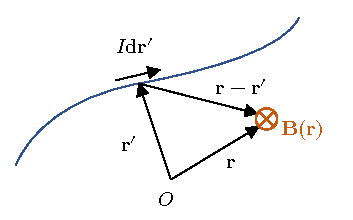
\includegraphics{magnetic_field_conductor_diff_view.pdf}
	\caption{Stromelement $I\diff\vec r$ und Magnetfeld $\vec B$ eines Leiterelements $\diff \vec r$. }
	\label{fig:magnetic_field_conductor_diff_view}
\end{figure}
Wir untersuchen zunächst die magnetische Flussdichte einiger speziellen geometrischen Anordnungen. Es gilt für ein Leiterelement $\diff \vec {r}'$ (dargestellt in \Abbref{fig:magnetic_field_conductor_diff_view}):
\begin{equation*}
	\diff \vec {B}=\frac{\mu _{0}}{4\pi }I\diff \vec {r}'\times \frac{\vec {r}-\vec {r}'}{\left| \vec {r}-\vec {r}'\right| ^{3}}
\end{equation*}
Dieser Zusammenhang ist als Biot-Savartsches Gesetz für Leiter bekannt und ergibt sich aus den Betrachtungen $\left| \diff \vec {B}\right| \propto I\left| \diff \vec {r}'\right| , \left| \vec {r}-\vec {r}'\right| ^{-2}$ und $\diff \vec {B}\perp \diff \vec {r}',\vec {r}-\vec {r}'$. Hier wird außerdem die magnetische Feldkonstante $\mu _{0}\approx 4\pi \cdot 10^{-7}\,\si{\newton\per\square\ampere}$ eingeführt\footnote{Über die Kraft zwischen zwei stromdurchflossene parallele Leiter wurde früher die Einheit Ampère definiert und dabei festgelegt, dass $\frac{\mu _{0}}{4\pi }=\SI{1e-7}{\newton\per\square\ampere}$, aber die magnetische Feldkonstante wurde 2019 umdefiniert auf Basis der Elementarladung und Sekunde, wobei aber die Abweichung extrem gering ist. Damit ist die magnetische Feldkonstante eine experimentell zu ermittelnde Größe geworden. }. Die Flussdichte ist zwar proportional zu $r^{-2}$ wie beim elektrischen Feld einer Punktladung, aber im Gegensatz können isolierte Stromelemente $I\diff \vec {r}$ nicht existieren.

Für das Feld eines unendlich langen, geraden Leiters gilt
\begin{equation*}
    \label{eq:biot_savart}
	B\left(\rho \right)=\frac{\mu _{0}}{4\pi }I\rho \int _{-\infty }^{\infty }\frac{\diff z}{\left(\rho ^{2}+z^{2}\right)^{\frac{3}{2}}}=\frac{\mu _{0}}{4\pi }\frac{I}{\rho },
\end{equation*}


\begin{figure}[htb]
	\centering
	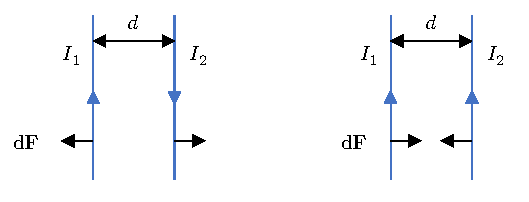
\includegraphics{force_parallel_conductors.pdf}
	\caption{Die Kraft auf parallele, stromdurchflossene Leiter ist anziehend, wenn der Stromfluss in verschiedene Richtungen geht und abstoßend, wenn der Strom in beiden Leiter in der gleichen Richtung fließt. }
	\label{fig:force_parallel_conductors}
\end{figure}

Diese Gleichung beschreibt das historische Biot-Savartsche Gesetz.

Verwendet man Gleichungen \eqref{eq:def_magn_flussdichte} und \eqref{eq:biot_savart}, so erhält man die Kraft zwischen zwei parallelen Leitern mit Abstand $d$ (siehe \Abbref{fig:force_parallel_conductors})
\begin{equation*}
    \frac{\diff\vec F}{\diff z} = \frac{\mu_0}{2\pi} \frac{I_1I_2}d,
\end{equation*}
die orthogonal zum Leiter ist.

Bis zum 20.5.2019 war der Ampère definiert als der Strom, der durch zwei parallele Leiter der Länge $\SI{1}{\m}$ mit $\SI{1}{\m}$ Abstand in gleicher Richtung fließt und eine Anziehungskraft von $\SI{1e-7}{\newton}$ bewirkt. 

Heute gilt
\begin{equation*}
	\SI{1}{\ampere}\equiv \frac{\SI{1}{\coulomb}}{\SI{1}{\s}}.
\end{equation*}
Zwischen beliebigen Leiterschleifen $C_{1},C_{2}$ wirkt eine Kraft von
\begin{equation*}
	\vec {F}_{21}=-\vec {F}_{12}=-\frac{\mu _{0}}{4\pi }I_{1}I_{2}\oint _{C_{1}}\oint _{C_{2}}\frac{\vec {r}_{1}-\vec {r}_{2}}{\left| \vec {r}_{1}-\vec {r}_{2}\right| ^{3}}\diff \vec {r}_{1}\cdot \diff \vec {r}_{2}.
\end{equation*}



\section{Grundgleichungen der Magnetostatik}

Um die Grundgleichungen der Magnetostatik herzuleiten, gehen wir zuerst von dem Stromelement $I\diff \vec {r}$ über in die Stromdichte $\vec {j}\left(\vec {r}\right)$ mit $I\diff \vec {r}=\vec {j}\left(\vec {r}\right)\diff^3 \vec {r}$.

Die Kraft auf ein Stromgebiet ist das Integral der Kraftdichte
\begin{equation*}
	\vec {F}=\int f\left(\vec {r}\right)\diff ^{3}\vec {r}=\int \vec {j}\left(\vec {r}\right)\times \vec {B}\left(\vec {r}\right)\diff ^{3}\vec {r}.
\end{equation*}
Für eine Punktladung $q$, die sich mit Geschwindigkeit $\vec {v}$ bewegt ($\vec {j}=q\vec {v}\delta \left(\vec {r}-\vec {r}\left(t\right)\right)$) gilt speziell
\begin{equation*}
	\vec F\left(\vec {r}\right)=q\vec {v}\times \vec {B}\left(\vec {r},t\right)
\end{equation*}
bzw. allgemein mit einem zusätzlichen elektrischen Feld
\begin{equation*}
	\vec F\left(\vec {r}\right)=q\left(\vec {v}\times \vec {B}\left(\vec {r},t\right)+\vec {E}\left(\vec {r},t\right)\right).
\end{equation*}
Diese Gesamtkraft ist die sogenannte Lorentzkraft.

Integration des Biot-Savartschen Gesetzes für Leiter führt auf\footnote{vergleichlich mit $\vec {E}(\vec r)=\frac{1}{4\pi \varepsilon _{0}}\int \rho \left(\vec {r}\right)\frac{\vec {r}-\vec {r}'}{\left| \vec {r}-\vec {r}'\right| ^{3}}\diff ^{3}\vec {r}'$.}
\begin{equation*}
	\vec {B}\left(\vec {r}\right)=\frac{\mu _{0}}{4\pi }\int \vec {j}\left(\vec {r'}\right)\times \frac{\vec {r}-\vec {r}'}{\left| \vec {r}-\vec {r}'\right| ^{3}}\diff ^{3}\vec {r}'.
\end{equation*}
Wie für das elektrische Feld können wir ein Potential einführen \textendash{} allerdings ist $\vec {B}$ kein Potentialfeld und daher ist das magnetische Potential ein Vektorpotential:
\begin{equation*}
	\vec {B}\left(\vec {r}\right)=\nabla \times \vec {A}\left(\vec {r}\right), \quad\vec {A}\left(\vec {r}\right)=\frac{\mu _{0}}{4\pi }\int \frac{\vec {j}\left(\vec {r}'\right)}{\left| \vec {r}-\vec {r}'\right| }\diff ^{3}\vec {r}'
\end{equation*}
Die Divergenz von $\vec {B}$ verschwindet, weil stets gilt, dass $\nabla\cdot(\nabla\times \vec A) = 0$.
\begin{formal}
		Das Magnetfeld hat keine Quellen, $\divg \vec {B}=0$.
\end{formal}
In der integralen Formulierung,
\begin{equation*}
	\int _{V}\divg \vec {B}\,\diff ^{3}\vec {r}=\int _{V}\vec {B}\cdot \diff \vec {f}=0,
\end{equation*}
bedeutet das, dass die magnetischen Feldlinien geschlossen sind. Es gibt folglich keine magnetischen Ladungen, wo die Feldlinien beginnen oder enden.

Für die Rotation der elektrischen Flussdichte gilt
\begin{align}
\begin{split}
    \label{eq:durchflutungsgesetz_magnetostatik}
	\rot \vec {B}&=\nabla \times \left(\nabla \times \vec {A}\right)=\nabla \left(\nabla \cdot \vec {A}\right)-\nabla ^{2}\vec {A}\\
	&=\frac{\mu _{0}}{4\pi }\nabla \int \vec {j}\left(\vec {r}'\right)\cdot \nabla \frac{1}{\left| \vec {r}-\vec {r}'\right| }\diff ^{3}\vec {r}'-\frac{\mu _{0}}{4\pi }\int \vec {j}\left(\vec {r}'\right)\nabla ^{2}\frac{1}{\left| \vec {r}-\vec {r}'\right| }\diff ^{3}\vec {r}'\\
	&=0+\mu _{0}\int \vec {j}\left(\vec {r}'\right)\delta \left(\vec {r}-\vec {r}'\right)\diff ^{3}\vec {r}'\\&=\mu _{0}\vec {j}\left(\vec {r}\right).
\end{split}
\end{align}

\begin{formal}
	Elektrische Ströme rufen Wirbel in der magnetischen Flussdichte hervor, $\rot \vec {B}=\mu _{0}\vec {j}\left(\vec {r}\right)$.
\end{formal}
Alternativ kann man sagen, dass die Zirkulation entlang der Oberfläche eines Volumens einem Strom durch das Volumen entspricht,
\begin{equation*}
	\boxed{\int _{\partial F}\vec {B}\cdot \diff \vec {r}=\mu _{0}I.}
\end{equation*}
Diese Gleichung ist als Ampèresches Gesetz bekannt. Mit seiner Nutzung kann man leicht das Magnetfeld von einem homogen stromdurchflossenen, zylindrischen Draht mit Radius $R$ bestimmen, wie in Abbildung \Abbref{fig:cylinder_conductor_with_diagrams} gezeigt. Wähle dazu eine kreisförmige Kurve $C$ mit Radius $r$ um die $z$-Achse herum. Aufgrund der Zylindersymmetrie ist das Magnetfeld nur vom Abstand $r$ der $z$-Achse abhängig und es gilt mit dem Ampèreschen Gesetz
\begin{align*}
		B\left(r\right)\oint _{C}1\diff s&=2\pi rB\left(r\right)=\mu _{0}I\left(r\right) \\
		\Leftrightarrow B\left(r\right)&=\frac{\mu _{0}I\left(r\right)}{2\pi r}.
\end{align*}


\begin{figure}[htb]
	\centering
	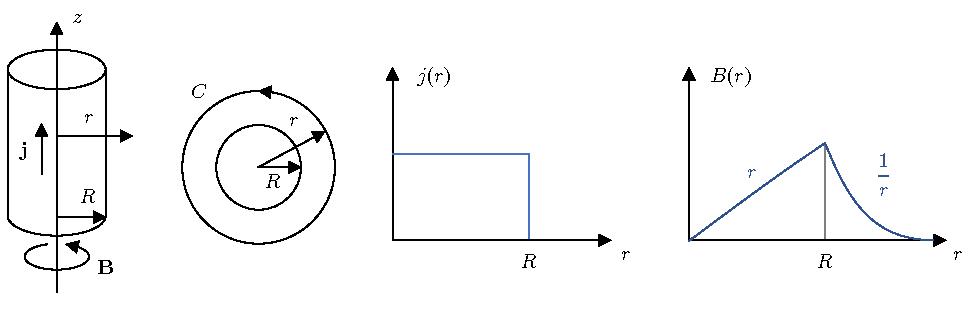
\includegraphics{cylinder_conductor_with_diagrams.pdf}
	\caption{Ein stromdurchflossener, zylindrischer Leiter mit Radius $R$ und Stromdichte $r$ erzeugt ein magnetisches Wirbelfeld. Links: schematische Darstellung, Mitte links: Querschnitt mit gedachter kreisförmiger Kurve $C$ mit Radius $r$ um den Leiter herum, Mitte rechts: Die Stromdichte ist konstant im Leiter und fällt außerhalb auf $0$ ab, rechts: im Leiter steigt der Betrag des Magnetfelds linear mit dem Abstand an und fällt außerhalb ab mit $r^{-1}$.  }
	\label{fig:cylinder_conductor_with_diagrams}
\end{figure}

Der Strom $I\left(r\right)$ enthält nur den Strom, der innerhalb der Kurve $C$ fließt. Innerhalb des zylindrischen Leiters ($r\leq R$) ist die eingeschlossene Fläche gerade $\pi r^{2}$ und damit
\begin{equation*}
	I\left(r\right)=j_{0}\pi r^{2}.
\end{equation*}


\begin{figure}[htb]
	\centering
	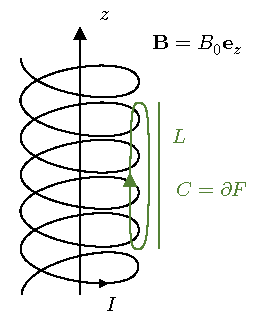
\includegraphics{long_coil_scheme.pdf}
	\caption{Magnetfeld einer lange, stromdurchflossenen Spule. }
	\label{fig:long_coil_scheme}
\end{figure}

Außerhalb des Leiters ist $I$ konstant $j_{0}\pi R^{2}$, weil sich der Leiter und damit der Stromfluss nur bis $r=R$ erstreckt. Das Magnetfeld ist also
\begin{align*}
	B\left(r\right)=\frac{\mu _{0}}{2}j_{0}\begin{cases} r,               & r\leq R \\
              \frac{R^{2}}{r}, & r>R
	                                       \end{cases}
\end{align*}
und es ist kreisförmig um die $z$-Achse gerichtet, $\vec {B}\left(r,\varphi \right)=B\left(r\right)\vec {e}_{\varphi }$.

Genauso lässt sich das Feld einer unendlich langen Spule berechnen (\Abbref{fig:long_coil_scheme}):
\begin{align*}
		\oint \vec {B}\cdot \diff \vec {r}&=LB_{0}\overset{!}{=}\mu _{0}NI \\
		\Rightarrow B_{0}&=\mu _{0}\frac{N}{L}I, \vec {B}=B_{0}\vec {e}_{z}
\end{align*}
Zwischen den Windungen hebt sich das magnetische Feld weg.

Wie aus der Gleichung \eqref{eq:durchflutungsgesetz_magnetostatik} hervorgeht, lässt sich für das Vektorpotential $\vec {A}$ wie in der Elektrostatik eine Poissongleichung formulieren,
\begin{equation*}
	\nabla ^{2}\vec {A}=-\mu _{0}\vec {j}
\end{equation*}
und im Potential $\vec {A}\left(\vec {r}\right)$ findet sich wieder eine Greenschen Funktion
\begin{equation*}
	\vec {A}\left(\vec {r}\right)=\int \diff ^{3}\vec {r}'G\left(\vec {r}-\vec {r}'\right)\vec {j}\left(\vec {r}'\right),\quad G\left(\vec {r}-\vec {r}'\right)=\frac{\mu _{0}}{4\pi }\frac{1}{\left| \vec {r}-\vec {r}'\right| }.
\end{equation*}
\section{Kleine Stromverteilungen: Der magnetische Dipol\label{mark-5.4}}

\subsection{Felder kleiner Stromverteilungen\label{mark-5.4.1}}

Wir führen zunächst wieder eine Entwicklung des magnetischen Potentials nach Momenten der Stromverteilung durch:
\begin{equation}
    \label{eq:entwicklung_magn_potential}
	\vec {A}\left(\vec {r}\right)=\frac{\mu _{0}}{4\pi }\int \diff ^{3}\vec {r}'\frac{\vec {j}\left(\vec {r}'\right)}{\left| \vec {r}-\vec {r}'\right| }\approx \frac{\mu _{0}}{4\pi }\left(\frac{1}{r}\int \diff ^{3}\vec {r}'\vec {j}\left(\vec {r}'\right)+\frac{\vec {r}}{r^{3}}\cdot \int \diff ^{3}\vec {r}'\vec {j}\left(\vec {r}'\right)\vec {r}'+\ldots \right)
\end{equation}
Die Auswertung ist allerdings viel komplizierter als für das elektrische Potential und daher beschränken wir uns hier auf die Dipole und vernachlässigen höhere Multipolmomente. Außerdem verwenden wir als Hilfsatz folgende Gleichung, die für beliebige skalare Felder $g$ und $f$ sowie für ein quellenfreies Vektorfeld $\vec {j}$ gilt\footnote{Beweis: Betrachte $\int _{V}\nabla \left(gf\vec {j}\right)\diff ^{3}\vec {r}$. Einerseits ist dieser Ausdruck mit dem Satz von Gauß gleich $\int _{\partial V}gf\vec {j}\cdot \diff \vec {f}$, was gleich $0$ ist, wenn man das Volumen groß genug wählt, dass auf dem Rand $\vec {j}\left(\vec {r}\right)=\vec {0}$ ist. Außerdem findet man mithilfe der Produktregel, dass $\int _{V}\nabla \left(gf\vec {j}\right)\diff ^{3}\vec {r}=\int _{V}\vec {j}\cdot \nabla \left(gf\right)\diff ^{3}\vec {r}+\int _{V}gf\nabla \cdot \vec {j}\diff ^{3}\vec {r}$, wobei der letzte Term aufgrund der Bedingung $\divg \vec {j}=\vec {0}$ verschwindet, q.e.d.}:
\begin{equation}
    \label{eq:hilfssatz}
	\int \vec {j}\cdot \nabla \left(gf\right)\diff ^{3}\vec {r}=0.
\end{equation}
Ferner können wir zeigen\footnote{Beweis: Mit der vorigen Formel $\int \vec {j}\cdot \nabla \left(gf\right)\diff ^{3}\vec {r}=0$ ist mit $g=1$ und $f=x_{i}$ offensichtlicherweise $\int j_{k}\cdot \nabla _{k}x_{i}\diff ^{3}\vec {r}=\int j_{i}\diff ^{3}\vec {r}=0$, q.e.d. }, dass
\begin{equation*}
	\int \vec {j}\left(\vec {r}\right)\diff ^{3}\vec {r}=0,
\end{equation*}
es also keine Strommonopole in $\vec {A}\left(\vec {r}\right)$ gibt. Als letzte Vorbereitung werten wir den zweiten Term in Gleichung \eqref{eq:entwicklung_magn_potential} aus
\begin{equation*}
	\vec {r}\cdot \int \diff ^{3}\vec {r}'\vec {j}\left(\vec {r}'\right)\vec {r}'=x_{i}\int \diff ^{3}\vec {r}'x_{i}^{'}j_{k}\left(\vec {r}'\right).
\end{equation*}
Das Produkt $T=x_{i}^{'}j_{k}$ ist ein Tensor zweiter Stufe und lässt sich zerlegen in einen symmetrischen und einen antisymmetrischen Teil, $T_{ik}=\frac{1}{2}\left(T_{ik}+T_{ki}\right)+\frac{1}{2}\left(T_{ik}-T_{ki}\right)$, also
\begin{equation*}
	\vec {r}\cdot \int \diff ^{3}\vec {r}'\vec {j}\left(\vec {r}'\right)\vec {r}'=x_{i}\int \diff ^{3}\vec {r}'\left(\frac{1}{2}\left(x_{i}^{'}j_{k}+x_{k}^{'}j_{i}\right)+\frac{1}{2}\left(x_{i}^{'}j_{k}-x_{k}^{'}j_{i}\right)\right).
\end{equation*}
Der erste Summand im Integranden (symmetrischer Teil des Tensors) verschwindet nach dem Hilfssatz \eqref{eq:hilfssatz} mit $g=x_{i}^{'},f=x_{k}^{'}$ und der zweite wird zu
\begin{equation*}
	\frac{1}{2}\int \diff ^{3}\vec {r}'\left(\left(\vec {r}\cdot \vec {r}'\right)\vec {j}-\left(\vec {r}\cdot \vec {j}\right)\vec {r}'\right)=\frac{1}{2}\int \diff ^{3}\vec {r}'\left(\vec {r}'\times \vec {j}\right)\times \vec {r}
\end{equation*}
evaluiert.

Nun können wir das magnetische Dipolmoment
\begin{equation*}
	\vec {m}=\frac{1}{2}\int \vec {r}'\times \vec {j}\left(\vec {r}\right)\diff ^{3}\vec {r}'
\end{equation*}
und das Vektorpotential des magnetischen Dipols
\begin{equation*}
	\vec {A}\left(\vec {r}\right)=\frac{\mu _{0}}{4\pi }\frac{\vec {m}\times \vec {r}}{r^{3}}
\end{equation*}
einführen. Daraus ergibt sich (mit weiteren Umformungen) schließlich das Magnetfeld eines Dipols
\begin{equation*}
	\vec {B}\left(\vec {r}\right)=\rot \vec {A}=-\frac{\mu _{0}}{4\pi }\nabla \frac{\vec {m}\cdot \vec {r}}{r^{3}}=\frac{\mu _{0}}{4\pi }\frac{3\left(\vec {m}\cdot \hat{\vec {r}}\right)\hat{\vec {r}}-\vec {m}}{r^{3}},
\end{equation*}
was wieder völlig analog zum elektrischen Dipol ist.

Wir wollen im Folgenden einmal das Dipolmoment zweier einfacher Geometrien berechnen. Das Dipolmoment einer Stromschleife (\Abbref{fig:magnetic_dipole_field_circle_conductor_ellipsoid}, links) ist einfach (verwende $\vec {j}\diff ^{3}\vec {r}=I\diff \vec {r}$)
\begin{equation*}
	\vec {m}=\frac{I}{2}\oint \vec {r}\times \diff \vec {r}.
\end{equation*}
Für eine ebene Schleife mit Fläche $F$ und Normalenvektor $\vec {n}$ (\Abbref{fig:magnetic_dipole_field_circle_conductor_ellipsoid}, Mitte) vereinfacht sich dieser Ausdruck zu
\begin{equation*}
	\vec {m}=IF\vec {n}.
\end{equation*}


\begin{figure}[htb]
	\centering
	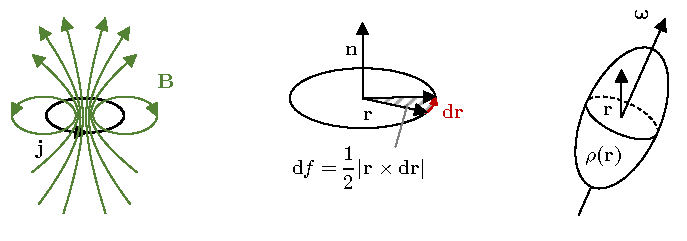
\includegraphics{magnetic_dipole_field_circle_conductor_ellipsoid.pdf}
	\caption{Links: Magnetfeld eines magnetischen Dipols, Mitte: Ein Kreisstrom erzeugt ein magnetisches Dipolmoment, rechts: starrer Körper, der mit $\vec\omega$ rotiert und einer Ladungsverteilung $\rho(\vec r)$ besitzt. }
	\label{fig:magnetic_dipole_field_circle_conductor_ellipsoid}
\end{figure}

Zuletzt betrachten wir einen starren geladenen Körper, der um eine Rotationsachse $\vec {\omega }$ rotiert (\Abbref{fig:magnetic_dipole_field_circle_conductor_ellipsoid}, rechts). Die lokale Geschwindigkeit für eine Ladung in diesem Körper ist $\vec {v}\left(\vec {r}\right)=\vec {\omega }\times \vec {r}$. Die rotierenden Ladungen resultieren in einer Stromdichte $\vec {j}=\rho \vec {v}$, sodass ein Dipolmoment induziert wird:
\begin{equation*}
	\vec {m}=\frac{1}{2}\int d^{3}\vec {r}\,\rho \left(\vec {r}\right)\vec {r}\times \vec {v}.
\end{equation*}
Gleichzeitig besitzt der Körper einen Drehimpuls
\begin{equation*}
	\vec {L}=\int \diff ^{3}\vec {r}\rho _{m}\left(\vec {r}\right)\vec {r}\times \vec {v}.
\end{equation*}
Trifft man jetzt die Annahme, dass die Verteilungen von Ladung und Masse im Körper gleich sind,
\begin{equation*}
	\frac{\rho \left(\vec {r}\right)}{\rho _{m}\left(\vec {r}\right)}=\frac{q_{\mathrm{ges}}}{m_{\mathrm{ges}}}\equiv \frac{q}{M},
\end{equation*}
dann findet man eine Proportionalität von $\vec {m}$ und $\vec {L}$:
\begin{equation*}
	\vec {m}=\frac{q}{2M}\vec {L}
\end{equation*}
Der Proportionalitätsfaktor $\left| \vec {m}\right| /\left| \vec {L}\right| $ wird als gyromagnetisches Verhältnis bezeichnet. Für den Spin gibt es allerdings eine Abweichung, die aus der Relativitätstheorie hervorgeht und es gilt eigentlich
\begin{equation*}
	\vec {m}=g\frac{q}{2M}\vec {L}
\end{equation*}
mit einem zusätzlichen Landé-Faktor (oder g-Faktor), dessen Wert von der Teilchensorte abhängt. Für Elektronen ist $g\approx 2$, für Protonen $g\approx 2\cdot 2,79$ und für Neutronen $g\approx 2\cdot \left(-1,91\right)$.

Auch die Erde ist ein magnetischer Dipol, der durch Ströme im flüssigen äußeren Erdkern angetrieben wird. Bemerkenswerterweise ist die Dipolachse leicht gegen die Erdachse geneigt und die Polarität dreht sich rund alle 200.000 Jahre um. Der Mechanismus ist allerdings bis heute nicht genau verstanden.

\subsection{Kraft, Drehmoment und Energie\label{mark-5.4.2}}

Die bereits bekannte Kraft auf ein Volumen $V$ mit Stromverteilung $\vec {j}\left(\vec {r}\right)$
\begin{equation*}
	\vec {F}=\int \vec {j}\left(\vec {r}\right)\times \vec {B}\left(\vec {r}\right)\diff ^{3}\vec {r}
\end{equation*}
lässt sich nach $\vec {B}$ um $\vec {r}=\vec {0}$ Taylor-entwickeln:
\begin{equation*}
	\vec {F}\approx \int \vec {j}\left(\vec {r}\right)\times \left(\vec {B}\left(0\right)+\vec {r}\cdot \nabla \vec {B}\left(0\right)+\ldots \right)\diff ^{3}\vec {r}=\left(\vec {m}\times \nabla \right)\times \vec {B}\left(0\right)=\nabla \left(\vec {m}\cdot \vec {B}\right)
\end{equation*}
Die potentielle Energie eines Dipols $\vec {m}$ im magnetischen Feld $\vec {B}$ ergibt sich daraus durch Integration
\begin{equation*}
	F=-\nabla U\Rightarrow U=-\vec {m}\cdot \vec {B}.
\end{equation*}
Das Minimum wird für $\vec {m}\upuparrows \vec {B}$ erreicht\footnote{vgl. Funktionsweise von einem Kompass. }. $U$ enthält aber nicht die Energie um den Dipol $\vec {m}$ aufrechtzuerhalten!

Das Drehmoment hat die gleiche Form wie für elektrische Dipole,
\begin{equation*}
	\vec {M}=\vec {m}\times \vec {B}
\end{equation*}
und auch die Wechselwirkungsenergie für einen Dipol im Feld eines zweiten Dipols ist analog
\begin{equation*}
	U=-\frac{\mu _{0}}{4\pi }\frac{3\left(\vec {m}_{1}\cdot \hat{\vec {r}}\right)\left(\vec {m}_{2}\cdot \hat{\vec {r}}\right)-\vec {m}_{1}\cdot \vec {m}_{2}}{r^{3}}.
\end{equation*}


